\section{Conceptos}
\frame
{
\frametitle{Conceptos}
\framesubtitle{OO}
\begin{itemize}
	\item Es importante que recordemos la \blue{Orientación a Objetos}.
	\item Es de \red{vital} importancia, para Python y para Qt.
\end{itemize}
}

\frame
{
\frametitle{Conceptos}
\framesubtitle{Jerarquía}
\begin{itemize}
	\item Su estructura es \blue{modular}.
	\begin{itemize}
		\item $>$ 300 clases.
		\item $>$ 6000 métodos.
	\end{itemize}
	\item En los cuales podemos encontrar:
	\begin{itemize}
		\item QtCore
		\item QtGui
		\item QtSvg
		\item QtSQL
		\item ...
	\end{itemize}
\end{itemize}
}

\frame
{
\frametitle{Conceptos}
\framesubtitle{Comportamiento}
\begin{itemize}
	\item Tenemos \blue{Objetos} (elementos)
	\item Tenemos \red{Señales} (por cada elemento) 
\end{itemize}
}

\frame
{
\frametitle{Conceptos}
\framesubtitle{Comportamiento}
\begin{center}
	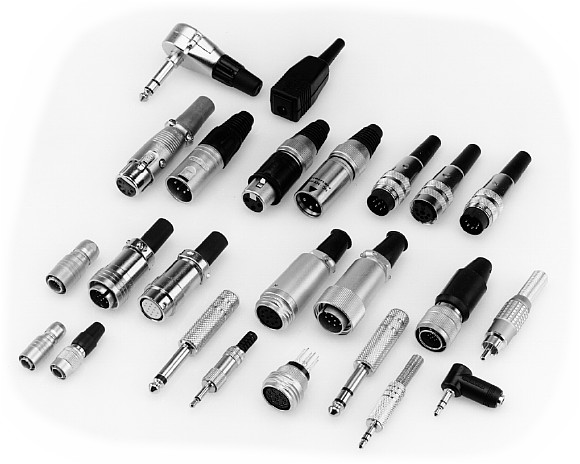
\includegraphics[width=0.5\textwidth]{img/tipos}
\end{center}
}

\frame
{
\frametitle{Conceptos}
\framesubtitle{Comportamiento}
\begin{itemize}
	\item Cada objeto tiene \blue{una o más} señales:
	\begin{itemize}
		\item \emph{connect()}
		\item \emph{valueChanged()}
		\item \emph{textChanged()}
		\item \emph{accepted()}
		\item \emph{triggered()}
		\item ...
	\end{itemize}
\end{itemize}
}
